\subsection{Edge Configurations, String Operators, and Equivalence Classes}\label{sec:density-matrix-whole}

To make the following discussions more fluent and precise, we denote by $\mathfrak{D}$ the \textit{edge configurations}, which are sets consisting of edges of a honeycomb lattice, and define their \textit{symmetric difference} $\oplus$ as
\[
\mathfrak{D}\oplus\mathfrak{D}' \equiv \mathfrak{D}\cup\mathfrak{D}'-\mathfrak{D}\cap\mathfrak{D}'\]
It can be directly verified to be commutative $\mathfrak{D}\oplus\mathfrak{D}' = \mathfrak{D}'\oplus\mathfrak{D}$ and associative $\lr{\mathfrak{D}_1\oplus\mathfrak{D}_2}\oplus\mathfrak{D}_3 = \mathfrak{D}_1\oplus\lr{\mathfrak{D}_2\oplus\mathfrak{D}_3}$. This algebra has three other properties, (i) $\varnothing\oplus\varnothing = \varnothing$, (ii) $\varnothing\oplus\mathfrak{D}=\mathfrak{D}$, and (iii) $\mathfrak{D}\oplus\mathfrak{D} = \varnothing$, which make it similar to the addition $\mathbb{Z}_2$. An example that illustrates the rule is given below
\[
\wordfig{2.5}{figures/oplus_1}\oplus\wordfig{2.5}{figures/oplus_2} = \wordfig{2.5}{figures/oplus_result},
\]
where thick red edges are those in the edge configurations.

With these, we define \emph{string operators} $\Sigma_\mathfrak{D}$ corresponding to different configurations $\mathfrak{D}$
\begin{equation}\label{equ.string-operator-def}
    \Sigma_\mathfrak{D} \equiv \prod_{\anglelr{ij}\in \mathfrak{D}}\sigma^{\alpha_{ij}}_i\sigma_j^{\alpha_{ij}}
\end{equation}
Because of the anti-commuting feature of the Pauli matrices, we have to notice the order of the product. For example, consider two connected edges. One of them, $\Sigma_{\anglelr{ij}}=\sigma_i^x\sigma_j^x$, is type-$x$, and the other, $\Sigma_{\anglelr{jk}}=\sigma^y_j\sigma^y_k$, is type-$y$. They share a common endpoint $j$. If we want to build $\Sigma_{\anglelr{ij}\oplus\anglelr{jk}}$, we will find that $\lr{\sigma^x_i\sigma_j^x}\lr{\sigma_j^y\sigma_k^y}$ and $\lr{\sigma^x_i\sigma_j^x}\lr{\sigma_j^y\sigma_k^y}$ are different in sign. This example illustrates that the order in which those dimers $\lr{\sigma^{\alpha_{ij}}_i\sigma^{\alpha_{ij}}_j}$ are placed in the product is important in several cases. To make the definition of string operators unique and self-consistent, we have to fix the order. In the subsequent discussion, we assume that all products include ordering information, such that every string operator is uniquely defined. 

A string operator $\Sigma_{\mathfrak{D}}$ is composed of $\mathbb{Z}_2$ dimer operators $\dimer{i}{j}$ within the edge configuration $\mathfrak{D}$. Therefore, multiplying two string operators $\Sigma_{\mathfrak{D}}$ and $\Sigma_{\mathfrak{D}}$ results in a symmetric difference pattern of the two edge configurations $\Sigma_{\mathfrak{D}\oplus\mathfrak{D}'}$. An equivalent statement is that the product of string operators represents the edge configuration algebra $\anglelr{\lrg{\mathfrak{D}},\oplus}$. More precisely, it gives a projective representation with a phase factor $g(\mathfrak{D},\mathfrak{D}')=\pm 1$,
\begin{equation}\label{equ.Sigma-representation}
\Sigma_{\mathfrak{D}}\Sigma_{\mathfrak{D}'} = g(\mathfrak{D},\mathfrak{D}') \Sigma_{\mathfrak{D}\oplus\mathfrak{D}'}.
\end{equation}


Compared to the open strings with endpoints, edge configurations composed of closed loops form a special class, since the expectation values of their corresponding string operators are equal to 1. For example, the simplest closed loop $\de p$ consists of six edges surrounding a plaquette $p$, and the corresponding string operator 
\[
\Sigma_{\de p} = \prod_{\anglelr{ij}\in\de p}\sigma^{\alpha_{ij}}_i\sigma^{\alpha_{ij}}_j = W_p
\]
is a plaquette operator $W_p$ centered at $p$. From the property of $W_p$, string operators of larger loops, as well as edge configurations consisting of multiple loops, can be expressed as combinations of plaquette operators in a specific set $\mathcal{A}$ of plaquettes, in which the loop is exactly the boundary of such a region,
\begin{equation}\label{equ.lattice-Stokes}
    \Sigma_{\de\mathcal{A}} = \prod_{p\in\mathcal{A}}W_p
\end{equation}
as illustrated in \autoref{fig.equivalent}. This is the lattice $\mathbb{Z}_2$ version of the Stokes theorem. As we know, the Kitaev ground state is an eigenvector of plaquette operators with an eigenvalue $+1$. That is, the expectation value of a string operator is equal to one whenever the edge configuration consists of closed loops without open strings. In conclusion, the expectation value of the string operator of the configuration $\mathfrak{D}$ is equal to another configuration $\mathfrak{D}\oplus\de\mathcal{A}$ constructed by adding a loop configuration $\de\mathcal{A}$ to the original one,
\[
\abs{\anglelr{\Sigma_{\de\mathcal{A}}\Sigma_{\mathfrak{D}}}} = \abs{\anglelr{\Sigma_{\mathfrak{D}}}} = \abs{\anglelr{\Sigma_{\de\mathcal{A}\oplus\mathfrak{D}}}}
\]
up to a sign. Such an equation is equivalent to 
\begin{equation}\label{equ.one-loop-equivalence}
\prod_{p\in\mathcal{A}}W_p\anglelr{\Sigma_{\de\mathcal{A}\oplus\mathfrak{D}}}\Sigma_{\de\mathcal{A}\oplus\mathfrak{D}} = \anglelr{\Sigma_{\mathfrak{D}}}\Sigma_{\mathfrak{D}}
\end{equation}
for an arbitrary set $\mathcal{A}$ of plaquettes. Notice that the sign need not be considered since any sign change in the expectation value is exactly canceled by the contribution from the string operator. Although equation \eqref{equ.one-loop-equivalence} shows that two configurations can be related by the loop operator $\Sigma_{\de \mathcal{A}}=\prod_{p\in\mathcal{A}}W_p$, it is not a general formula to relate all kinds of equivalent edge configurations in a unified way. Fortunately, the loop operator $\prod_{p\in\mathcal{A}}W_p$ is composed by $\mathbb{Z}_2$ operators $W_p$, and we also know that the projector $\mathcal{P}^{(p)}$ defined as
\begin{equation}\label{equ.p-projector}
    \mathcal{P}^{(p)}\equiv\prod_{p}\lr{\frac{\mathds{1}+W_p}{2}}
\end{equation}
is invariant after being multiplied by an operator $W_p$
\[
\mathcal{P}^{(p)}W_{p} = \mathcal{P}^{(p)}
\]
This equation can be understood as the plaquette operator $W_{p}$ being absorbed into the projector, and is equivalent to doing nothing. For the same reason, we also have the following relation
\[
\mathcal{P}^{(p)}\prod_{p\in\mathcal{A}}W_p = \mathcal{P}^{(p)}
\]
for arbitrary plaquette configurations $\mathcal{A}$. Combining this relation with \eqref{equ.one-loop-equivalence}, we then have a more general equation to relate the configuration $\mathfrak{D}$ and $\mathfrak{D}\oplus\de\mathcal{A}$,
\begin{equation}\label{equ.string-operator-equivalent}
\mathcal{P}^{(p)}\anglelr{\Sigma_{\de\mathcal{A}\oplus\mathfrak{D}}}\Sigma_{\de\mathcal{A}\oplus\mathfrak{D}} 
= \mathcal{P}^{(p)}\anglelr{\Sigma_{\mathfrak{D}}}\Sigma_{\mathfrak{D}}
\end{equation}

\begin{figure}
    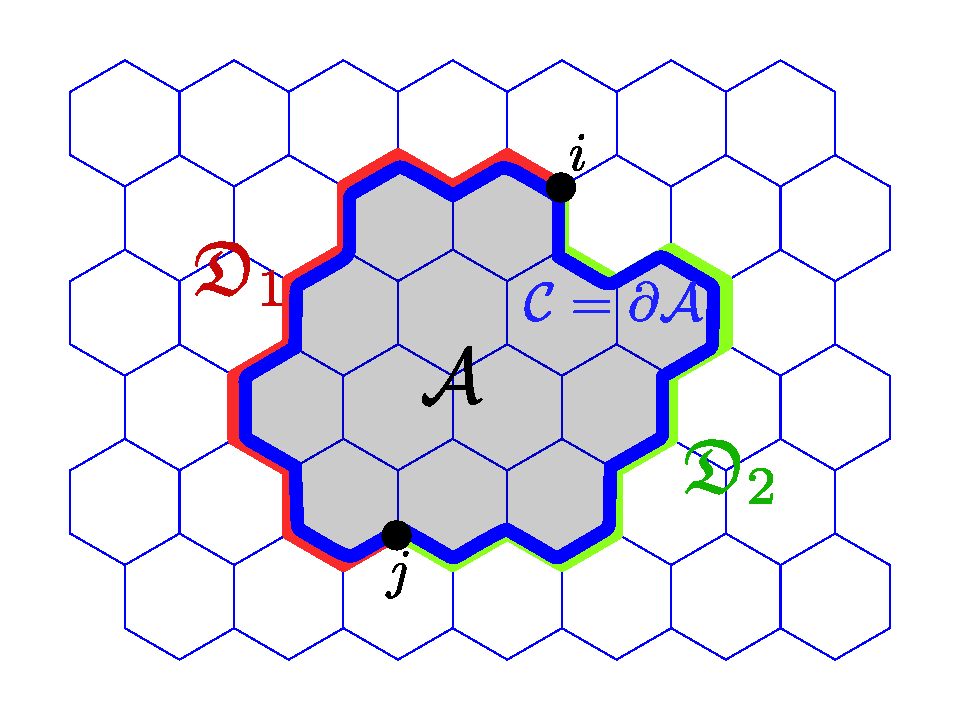
\includegraphics[width=0.45\linewidth]{figures/equivalent_loop.pdf}
    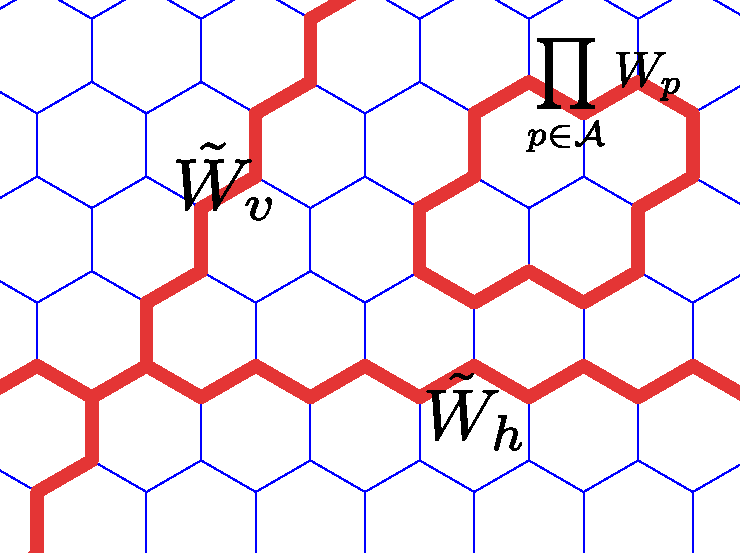
\includegraphics[width=0.45\linewidth]{figures/equivalent.pdf}
    \caption{The left panel shows two equivalent edge configurations $\mathfrak{D}_1\sim\mathfrak{D}_2$ bridged via a loop $\mathcal{C}=\de\mathcal{A}$. The two configurations share the same endpoints $i$ and $j$. The right panel shows three possible ways to get other dimer configurations with the same expectation value of the string operators. The two Wilson loops, $\Tilde{W}_h\equiv \Sigma_{\mathcal{L}_h}$ and $\Tilde{W}_v\equiv \Sigma_{\mathcal{L}_v}$ commute $[\Tilde{W}_h,\Tilde{W}_v]=0$, and neither of them can be constructed by local operators $W_p$'s. Aside from the global Wilson loops, we also have local ones, given by plaquette operators $ W_p$ inside the region $\mathcal{A}$.}
    \label{fig.equivalent}
\end{figure}
Equations~\eqref{equ.one-loop-equivalence} and \eqref{equ.string-operator-equivalent} imply an equivalence relation for edge configurations defined in such a way that two edge configurations $\mathfrak{D}_1$ and $\mathfrak{D}_2$ are \emph{equivalent}, denoted by $\mathfrak{D}_1\sim\mathfrak{D}_2$, if and only if there exists a set $\mathcal{A}$ of plaquettes such that one of the following four conditions holds:
\begin{enumerate}
    \item[(i)] $\mathfrak{D}_1=\mathfrak{D}_2\oplus\de\mathcal{A}$
    \item[(ii)] $\mathfrak{D}_1=\mathfrak{D}_2\oplus\de\mathcal{A}\oplus\mathcal{L}_v$
    \item[(iii)] $\mathfrak{D}_1=\mathfrak{D}_2\oplus\de\mathcal{A}\oplus\mathcal{L}_h$
    \item[(iv)] $\mathfrak{D}_1=\mathfrak{D}_2\oplus\de\mathcal{A}\oplus\mathcal{L}_v\oplus\mathcal{L}_h$
\end{enumerate} 
$\mathcal{L}_v$ and $\mathcal{L}_h$ are the global loop that circles the torus in the vertical and horizontal directions, the corresponding string operators of which are $\Tilde{W}_v\equiv\Sigma_{\mathcal{L}_v}$ and $\Tilde{W}_h\equiv\Sigma_{\mathcal{L}_h}$, respectively, as illustrated in the right panel of \autoref{fig.equivalent}. Equivalent configurations are collected into \emph{equivalence classes} $[\mathfrak{D}^c]=\lrg{\mathfrak{D}:\mathfrak{D}\sim\mathfrak{D}^c}$ characterized by each character $\mathfrak{D}^c$. The right panel of Fig.~\ref{fig.equivalent} shows that the two equivalent edge configurations must share the same set of endpoints, giving a simple way to identify equivalent edge configurations. In other words, there is a one-to-one correspondence between an equivalence class for edge configurations $[\mathfrak{D}]$ and the \textit{set of endpoints} of the character configuration $\mathfrak{D}$, denoted by $\mrm{EP}\lr{\mathfrak{D}}$. 
\begin{figure}
    \centering
    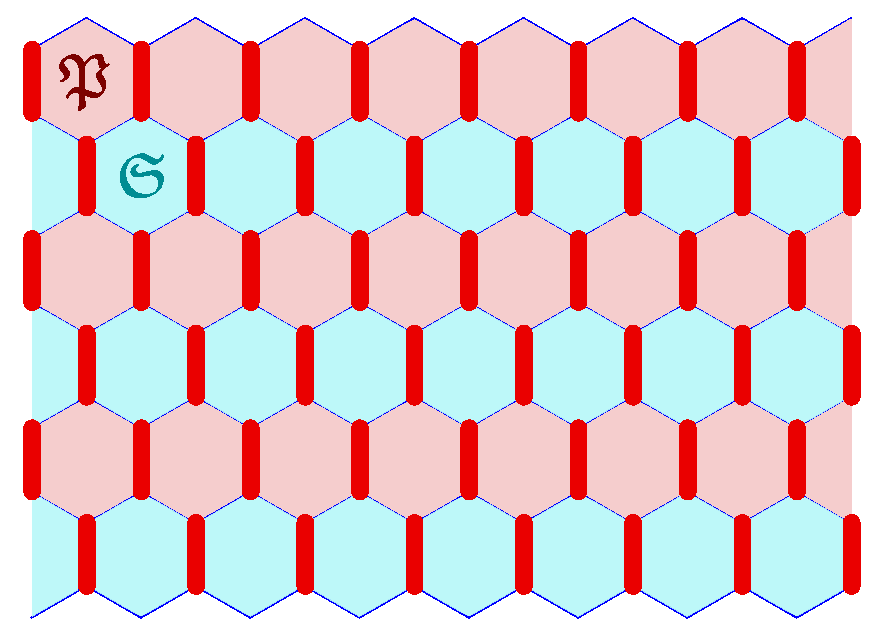
\includegraphics[width=0.48\linewidth]{figures/S-P-dimer-gas.pdf}
    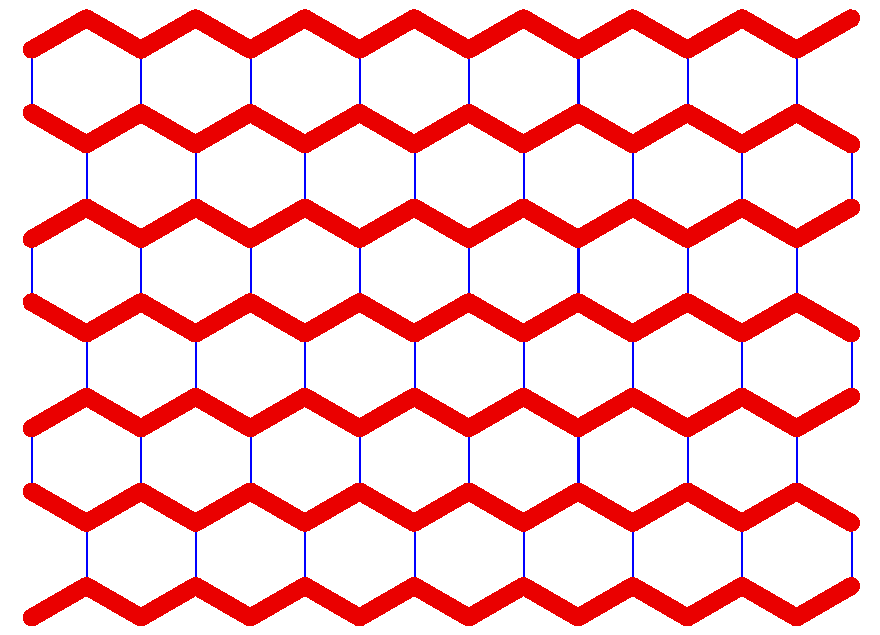
\includegraphics[width=0.48\linewidth]{figures/snake-and-dimer-gas.pdf}
    \caption{The left panel illustrates the plaqeutte configurations $\mathfrak{P}$ and $\mathfrak{S}$ as well as the edge configuration $\mathfrak{D}_Z$. The set of plaquettes in pink is denoted by $\mathfrak{P}$, while the set containing those in pink-blue is denoted by $\mathfrak{S}$. The edge configuration $\mathfrak{D}_Z$ consists of all of the red $z$-directional edges in the system, as shown in the above figure. The right panel illustrates the zigzag configuration $\mathfrak{D}_{zz}$ consisting of edges at all the horizontal loops. Such an edge configuration is also the boundary of both $\mathfrak{P}$ and $\mathfrak{S}$, for which we can write $\mathfrak{D}_{zz} = \de\mathfrak{P} = \de\mathfrak{S}$. Note that $\Sigma_{\mathfrak{D}_Z}=\Sigma_{\mathfrak{D}_{zz}}$ although $\mrm{EP}(\mathfrak{D}_Z)\neq \mrm{EP}(\mathfrak{D}_{zz})=\varnothing$} 
    \label{fig.S-P-dimer-gas}
\end{figure}

String operators of edge configurations in the same class have the same magnitude of expectation values,
\[
\abs{\anglelr{\Sigma_{\mathfrak{D}}}} = \abs{\anglelr{\Sigma_{\mathfrak{D}'}}} \quad\text{if $\mathfrak{D}\sim\mathfrak{D}'$}
\]
hence contribute the same weight to the density matrix. Nevertheless, it is still possible for two configurations from different classes to have the same weight contribution to the density matrix. There are a type of plaquette configurations, $\mathfrak{P}$ and $\mathfrak{S}$, that transform an edge configuration $\mathfrak{D}$ to $\mathfrak{D}\oplus\mathfrak{D}_Z$ because of the following relation
\begin{equation}\label{equ.P-S-dimer}
    \prod_{p\in\mathfrak{P}}W_p = \prod_{p\in\mathfrak{S}}W_p = \prod_{\anglelr{ij}\in \mathfrak{D}_Z}\sigma_i^z\sigma_{j}^z = \Sigma_{\mathfrak{D}_Z}.
\end{equation}
The plaquette configurations $\mathfrak{P}$ and $\mathfrak{S}$ as well as the edge configuration $\mathfrak{D}_Z$ are illustrated in the left panel of \autoref{fig.S-P-dimer-gas}. The edge configuration $\mathfrak{D}_Z$ is composed of the $z$-directional dimers all over the system. The plaquette configuration $\mathfrak{P}$ contains all the plaquettes at the even horizontal layers, while $\mathfrak{S}$ is the complement of $\mathfrak{P}$. The endpoint configuration $\mrm{EP}(\mathfrak{D}_Z)$ is simply the set of all the lattice sites in the system. On the other hand, the operators $\prod_{p\in\mathfrak{P}}W_p$ and $\prod_{p\in \mathfrak{S}}W_p$ is also equal to the string operator of the zigzag edge configuration $\mathfrak{D}_{zz}$, a set of all the $x$- and $y$-edges, as illustrated in the right panel of \autoref{fig.S-P-dimer-gas}
\begin{equation}\label{equ.M-MZ-complement}
\prod_{p\in\mathfrak{P}}W_p = \prod_{p\in\mathfrak{S}}W_p  = \Sigma_{\mathfrak{D}_{zz}}
\end{equation}
because $\de\mathfrak{P} = \de\mathfrak{S} = \mathfrak{D}_{zz}$.  Unlike $\mathfrak{D}_Z$, this edge configuration has no endpoints, $\mrm{EP}(\mathfrak{D}_{zz})=\varnothing$, and is equivalent to vacuum. So, we need to keep in mind that every two configurations, $\mathfrak{D}\oplus\mathfrak{D}_Z$ and $\mathfrak{D}\oplus\mathfrak{D}_{zz}$, give an identical string operator, although they are not equivalent.

We would also like to show that the physical meaning of the operator $\Sigma_{\mathfrak{D}_Z}$ is exactly the total fermion parity of the $c$-Majorana fermions. Because the expectation values of fluxes are fixed to be $\anglelr{W_p}=+1$ in the ground state, we directly know that the expectation value of $\Sigma_{\mathfrak{D}_Z}$ is equal to $+1$ directly from equation \eqref{equ.P-S-dimer} 
\begin{equation}\label{equ.fermion-parity-dimer-rep}
    \anglelr{\Sigma_{\mathfrak{D}_Z}}=1
\end{equation}
It is also worth mentioning that the combination of the plaquette operator over $\mathfrak{P}$ and the string operators containing $z$-dimers all over the lattice is equal to multiplying all edges in the entire lattice $\Lambda$ together
\begin{equation}\label{equ.fermion-parity-spin-rep}
    \lr{\prod_{p\in\mathfrak{P}}W_p} \Sigma_{\mathfrak{D}_Z} = \prod_{\anglelr{ij}\in\Lambda}\dimer{i}{j} = \mathds{1}
\end{equation}
This is nothing but the identity operator of the entire system because of the geometry of the honeycomb lattice. We can understand equations \eqref{equ.fermion-parity-dimer-rep} and \eqref{equ.fermion-parity-spin-rep} in the sense of fermion parity. In our convention, the gauge is fixed as $u_{ij}=1\forall\anglelr{ij}$, therefore, the string operator corresponding to the edge configuration that contains all of the edges in the lattice, as appeared in the last equation, transforms into the fermion parity operator $\hat{\bog{\pi}}$ up to a phase~\footnote{Two distinct Majorana fermions, say $c_1$ and $c_2$, can combine to form a normal fermion degree of freedom $f$ in a way that $f=\frac{1}{2}\lr{c_1+ic_2}$ and $f^\dagger=\frac{1}{2}\lr{c_1-ic_2}$. In this way, the fermion parity operator represented using the Majorana fermions becomes $\hat{\bog{\pi}}\equiv(-1)^{f^\dagger f}=ic_1c_2$. In a more general sense, the fermion parity operator is equal to the multiplication of all the Majorana fermions $\prod_i c_i$ up to a phase.}
\begin{equation}\label{equ.total-fermion-parity-entire-system}
    \prod_{\anglelr{ij}\in\Lambda}\dimer{i}{j}\to \prod_{\anglelr{ij}\in \Lambda}ic_ic_j
\propto \prod_{i\in\Lambda}c_i\propto \hat{\bog{\pi}}
\end{equation}
This is also due to the geometric feature of the honeycomb lattice, in which three connected edges share a lattice site. Similarly, the operator $\Sigma_{\mathfrak{D}_Z}$ in the Majorana representation is also equal to the fermion parity operator
\begin{equation}\label{equ.total-fermion-parity-Sigma-Z}
    \Sigma_{\mathfrak{D}_Z} \to \prod_{\anglelr{ij}\in\mathfrak{D}_Z}ic_ic_j\propto \prod_{i\in\Lambda}c_i\propto\hat{\bog{\pi}},
\end{equation}
because, as we will emphasize later, Majorana fermions emerge at the endpoints of each $z$-directional dimer, thus $\mrm{EP}(\mathfrak{D}_Z)$ is exactly the whole lattice system $\Lambda$. From the Majorana fermion point of view, the fermionic representation of the Kitaev Hamiltonian \eqref{equ.MF-Hamiltonian} is quadratic. As a consequence, the total fermion parity of the whole system should be conserved and must be $+1$ on a torus~\cite{Fu-Knolle-Perkins-2018}. This fermion parity degree of freedom is emergent only in the Majorana representation, and should be fixed by the intrinsic property of the spin operators in the physical spin representation. This is why the expectation value of the operator $\Sigma_{\mathfrak{D}_Z}$ is $+1$. 

Aside from the convenience arising from the fact that endpoint-point sets uniquely determine the equivalent class, the physical picture about the equivalence classes and endpoint sets also implies that a Pauli string in the spin representation is identical to the two Majorana fermions residing on the endpoints of the string. This can be seen in the \textit{commutation} among the endpoints of strings~\cite{Kitaev, fermion-and-string}. More details will be discussed in Section \ref{sec:Emergent-Fermions-at-the-Endpoints}. 

